

\tikzset{every picture/.style={line width=0.75pt}} %set default line width to 0.75pt        

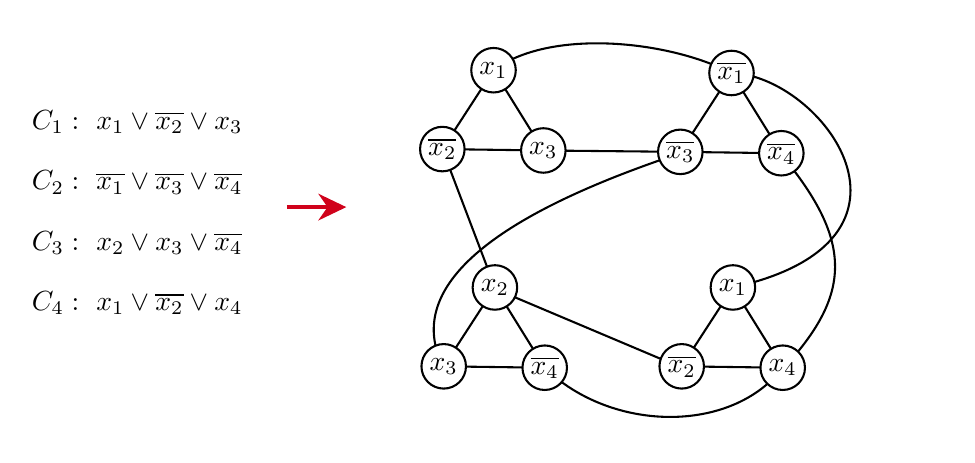
\begin{tikzpicture}[x=0.5pt,y=0.5pt,yscale=-1,xscale=1]
%uncomment if require: \path (0,313); %set diagram left start at 0, and has height of 313

%Straight Lines [id:da6618167296725836] 
\draw    (416.92,104.08) -- (515.92,105.08) ;
%Curve Lines [id:da22396963516709756] 
\draw    (589.92,261.08) .. controls (553,309) and (466,308) .. (417.92,261.08) ;
%Straight Lines [id:da4039573391796768] 
\draw    (343.92,103.08) -- (381.92,203.08) ;
%Straight Lines [id:da13937003486319577] 
\draw    (381.92,204.08) -- (516.92,261.08) ;
%Curve Lines [id:da866328606831125] 
\draw    (344.92,261.08) .. controls (308,190) and (420,138) .. (515.92,106.08) ;
%Curve Lines [id:da9209425626994789] 
\draw    (588.92,107.08) .. controls (642,171) and (639,209) .. (589.92,262.08) ;
%Curve Lines [id:da4940637759678749] 
\draw    (552.92,48.08) .. controls (618,50) and (708,169) .. (553.92,203.08) ;
%Curve Lines [id:da5522864666968264] 
\draw    (380.92,46.08) .. controls (420.92,16.08) and (506,24) .. (552.92,48.08) ;
%Straight Lines [id:da39949851653001356] 
\draw    (343.92,103.08) -- (416.92,104.08) ;
%Straight Lines [id:da06151606308920077] 
\draw    (380.92,46.08) -- (416.92,104.08) ;
%Straight Lines [id:da6053357926244952] 
\draw    (343.92,103.08) -- (380.92,46.08) ;
%Shape: Ellipse [id:dp6988649017460684] 
\draw  [fill={rgb, 255:red, 255; green, 255; blue, 255 }  ,fill opacity=1 ] (327.83,103.08) .. controls (327.83,94.19) and (335.03,86.99) .. (343.92,86.99) .. controls (352.8,86.99) and (360,94.19) .. (360,103.08) .. controls (360,111.96) and (352.8,119.16) .. (343.92,119.16) .. controls (335.03,119.16) and (327.83,111.96) .. (327.83,103.08) -- cycle ;
%Shape: Ellipse [id:dp6915506911604865] 
\draw  [fill={rgb, 255:red, 255; green, 255; blue, 255 }  ,fill opacity=1 ] (400.83,104.08) .. controls (400.83,95.19) and (408.03,87.99) .. (416.92,87.99) .. controls (425.8,87.99) and (433,95.19) .. (433,104.08) .. controls (433,112.96) and (425.8,120.16) .. (416.92,120.16) .. controls (408.03,120.16) and (400.83,112.96) .. (400.83,104.08) -- cycle ;
%Shape: Ellipse [id:dp4366461272272538] 
\draw  [fill={rgb, 255:red, 255; green, 255; blue, 255 }  ,fill opacity=1 ] (364.83,46.08) .. controls (364.83,37.19) and (372.03,29.99) .. (380.92,29.99) .. controls (389.8,29.99) and (397,37.19) .. (397,46.08) .. controls (397,54.96) and (389.8,62.16) .. (380.92,62.16) .. controls (372.03,62.16) and (364.83,54.96) .. (364.83,46.08) -- cycle ;
%Straight Lines [id:da042710010547382216] 
\draw    (515.92,105.08) -- (588.92,106.08) ;
%Straight Lines [id:da8892833055324549] 
\draw    (552.92,48.08) -- (588.92,106.08) ;
%Straight Lines [id:da0818748968414269] 
\draw    (515.92,105.08) -- (552.92,48.08) ;
%Shape: Ellipse [id:dp3629673290953376] 
\draw  [fill={rgb, 255:red, 255; green, 255; blue, 255 }  ,fill opacity=1 ] (499.83,105.08) .. controls (499.83,96.19) and (507.03,88.99) .. (515.92,88.99) .. controls (524.8,88.99) and (532,96.19) .. (532,105.08) .. controls (532,113.96) and (524.8,121.16) .. (515.92,121.16) .. controls (507.03,121.16) and (499.83,113.96) .. (499.83,105.08) -- cycle ;
%Shape: Ellipse [id:dp13012257517742154] 
\draw  [fill={rgb, 255:red, 255; green, 255; blue, 255 }  ,fill opacity=1 ] (572.83,106.08) .. controls (572.83,97.19) and (580.03,89.99) .. (588.92,89.99) .. controls (597.8,89.99) and (605,97.19) .. (605,106.08) .. controls (605,114.96) and (597.8,122.16) .. (588.92,122.16) .. controls (580.03,122.16) and (572.83,114.96) .. (572.83,106.08) -- cycle ;
%Shape: Ellipse [id:dp4087408185133151] 
\draw  [fill={rgb, 255:red, 255; green, 255; blue, 255 }  ,fill opacity=1 ] (536.83,48.08) .. controls (536.83,39.19) and (544.03,31.99) .. (552.92,31.99) .. controls (561.8,31.99) and (569,39.19) .. (569,48.08) .. controls (569,56.96) and (561.8,64.16) .. (552.92,64.16) .. controls (544.03,64.16) and (536.83,56.96) .. (536.83,48.08) -- cycle ;
%Straight Lines [id:da3279698789670312] 
\draw    (344.92,260.08) -- (417.92,261.08) ;
%Straight Lines [id:da13651038513236746] 
\draw    (381.92,203.08) -- (417.92,261.08) ;
%Straight Lines [id:da07037214338199449] 
\draw    (344.92,260.08) -- (381.92,203.08) ;
%Shape: Ellipse [id:dp040453670796765206] 
\draw  [fill={rgb, 255:red, 255; green, 255; blue, 255 }  ,fill opacity=1 ] (328.83,260.08) .. controls (328.83,251.19) and (336.03,243.99) .. (344.92,243.99) .. controls (353.8,243.99) and (361,251.19) .. (361,260.08) .. controls (361,268.96) and (353.8,276.16) .. (344.92,276.16) .. controls (336.03,276.16) and (328.83,268.96) .. (328.83,260.08) -- cycle ;
%Shape: Ellipse [id:dp4286753979995753] 
\draw  [fill={rgb, 255:red, 255; green, 255; blue, 255 }  ,fill opacity=1 ] (401.83,261.08) .. controls (401.83,252.19) and (409.03,244.99) .. (417.92,244.99) .. controls (426.8,244.99) and (434,252.19) .. (434,261.08) .. controls (434,269.96) and (426.8,277.16) .. (417.92,277.16) .. controls (409.03,277.16) and (401.83,269.96) .. (401.83,261.08) -- cycle ;
%Shape: Ellipse [id:dp772850742920124] 
\draw  [fill={rgb, 255:red, 255; green, 255; blue, 255 }  ,fill opacity=1 ] (365.83,203.08) .. controls (365.83,194.19) and (373.03,186.99) .. (381.92,186.99) .. controls (390.8,186.99) and (398,194.19) .. (398,203.08) .. controls (398,211.96) and (390.8,219.16) .. (381.92,219.16) .. controls (373.03,219.16) and (365.83,211.96) .. (365.83,203.08) -- cycle ;
%Straight Lines [id:da5751805739442735] 
\draw    (516.92,260.08) -- (589.92,261.08) ;
%Straight Lines [id:da5903012678345287] 
\draw    (553.92,203.08) -- (589.92,261.08) ;
%Straight Lines [id:da38407080032275986] 
\draw    (516.92,260.08) -- (553.92,203.08) ;
%Shape: Ellipse [id:dp5500860302509325] 
\draw  [fill={rgb, 255:red, 255; green, 255; blue, 255 }  ,fill opacity=1 ] (500.83,260.08) .. controls (500.83,251.19) and (508.03,243.99) .. (516.92,243.99) .. controls (525.8,243.99) and (533,251.19) .. (533,260.08) .. controls (533,268.96) and (525.8,276.16) .. (516.92,276.16) .. controls (508.03,276.16) and (500.83,268.96) .. (500.83,260.08) -- cycle ;
%Shape: Ellipse [id:dp9081445012691336] 
\draw  [fill={rgb, 255:red, 255; green, 255; blue, 255 }  ,fill opacity=1 ] (573.83,261.08) .. controls (573.83,252.19) and (581.03,244.99) .. (589.92,244.99) .. controls (598.8,244.99) and (606,252.19) .. (606,261.08) .. controls (606,269.96) and (598.8,277.16) .. (589.92,277.16) .. controls (581.03,277.16) and (573.83,269.96) .. (573.83,261.08) -- cycle ;
%Shape: Ellipse [id:dp7856009471528769] 
\draw  [fill={rgb, 255:red, 255; green, 255; blue, 255 }  ,fill opacity=1 ] (537.83,203.08) .. controls (537.83,194.19) and (545.03,186.99) .. (553.92,186.99) .. controls (562.8,186.99) and (570,194.19) .. (570,203.08) .. controls (570,211.96) and (562.8,219.16) .. (553.92,219.16) .. controls (545.03,219.16) and (537.83,211.96) .. (537.83,203.08) -- cycle ;
%Straight Lines [id:da14088417165595923] 
\draw [color={rgb, 255:red, 208; green, 2; blue, 27 }  ,draw opacity=1 ][line width=1.5]    (231.5,145) -- (270.5,145) ;
\draw [shift={(274.5,145)}, rotate = 180] [fill={rgb, 255:red, 208; green, 2; blue, 27 }  ,fill opacity=1 ][line width=0.08]  [draw opacity=0] (20.36,-9.78) -- (0,0) -- (20.36,9.78) -- (13.52,0) -- cycle    ;

% Text Node
\draw (45,73) node [anchor=north west][inner sep=0.75pt]   [align=left] {$\displaystyle C_{1} :\ x_{1} \lor \overline{x_{2}} \lor x_{3}$};
% Text Node
\draw (45,116.67) node [anchor=north west][inner sep=0.75pt]   [align=left] {$\displaystyle C_{2} :\ \overline{x_{1}} \lor \overline{x_{3}} \lor \overline{x_{4}}$};
% Text Node
\draw (45,160.34) node [anchor=north west][inner sep=0.75pt]   [align=left] {$\displaystyle C_{3} :\ x_{2} \lor x_{3} \lor \overline{x_{4}}$};
% Text Node
\draw (45,204) node [anchor=north west][inner sep=0.75pt]   [align=left] {$\displaystyle C_{4} :\ x_{1} \lor \overline{x_{2}} \lor x_{4}$};
% Text Node
\draw (380.92,46.08) node   [align=left] {$\displaystyle x_{1}$};
% Text Node
\draw (552.92,48.08) node   [align=left] {$\displaystyle \overline{x_{1}}$};
% Text Node
\draw (381.92,203.08) node   [align=left] {$\displaystyle x_{2}$};
% Text Node
\draw (343.92,103.08) node   [align=left] {$\displaystyle \overline{x_{2}}$};
% Text Node
\draw (416.92,104.08) node   [align=left] {$\displaystyle x_{3}$};
% Text Node
\draw (515.92,105.08) node   [align=left] {$\displaystyle \overline{x_{3}}$};
% Text Node
\draw (588.92,106.08) node   [align=left] {$\displaystyle \overline{x_{4}}$};
% Text Node
\draw (417.92,261.08) node   [align=left] {$\displaystyle \overline{x_{4}}$};
% Text Node
\draw (344.92,260.08) node   [align=left] {$\displaystyle x_{3}$};
% Text Node
\draw (553.92,203.08) node   [align=left] {$\displaystyle x_{1}$};
% Text Node
\draw (516.92,260.08) node   [align=left] {$\displaystyle \overline{x_{2}}$};
% Text Node
\draw (589.92,261.08) node   [align=left] {$\displaystyle x_{4}$};


\end{tikzpicture}

